\chapter{Einstellungen (brv)}
\label{chap:settings}

Über das Einstellugnsmenü lässt sich die App in zwei Punkten konfigurieren:

\begin{enumerate}
	\item Einstellung der Sprache (s. \cref{sec:lang})
	\item Einstellung der Eingabemethode (s. \cref{sec:input})
\end{enumerate}

Die Einstellungsseite wird je nach Ansicht, in der sich der Nutzer aktuell befindet, auf verschiedene Arten geöffnet:

\begin{enumerate}
	\item \textbf{Profilverwaltung:} Die AppBar der Profilverwaltung enthält einen Button, der aus einem Zahnrad-Icon besteht und per direktem Klick die Einstellungsansicht öffnet (s. \cref{img:openSettings} links).
	\item \textbf{Sonstige Ansichten:} Alle weiteren Ansichten (außer der Profilverwaltung) enthalten in der AppBar ein Dropdown (s. \cref{img:openSettings} Mitte), mithilfe dessen über den zweiten Menüpunkt die Einstellungsseite geöffnet werden kann (s. \cref{img:openSettings} rechts).
\end{enumerate}

\begin{figure}[H]
	\centering
	\begin{subfigure}[b]{0.3\textwidth}
		\centering
		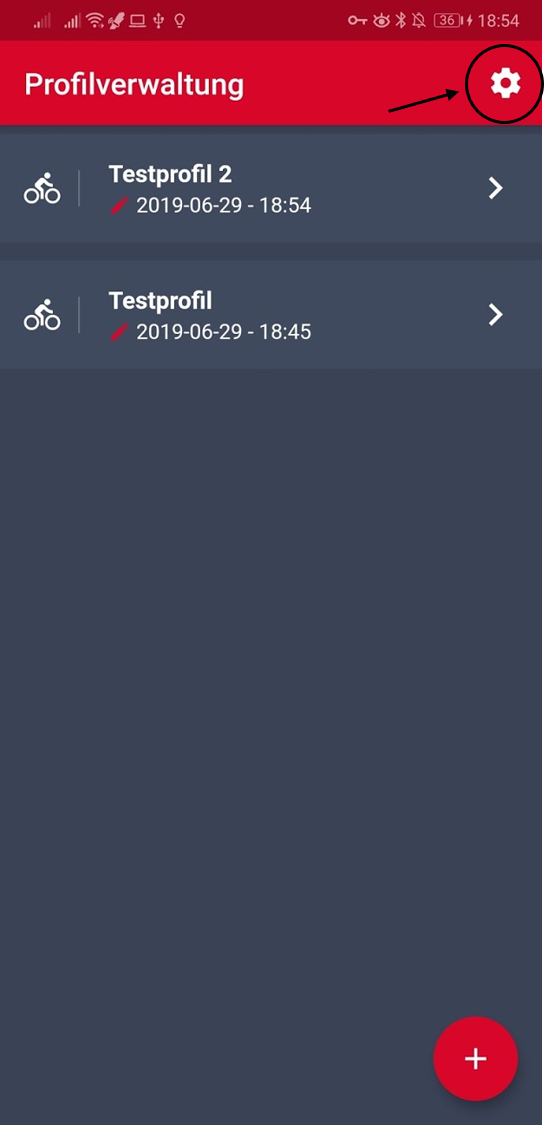
\includegraphics[width=1\textwidth]{../include/images/settings/Open_Settings_01}
	\end{subfigure}
	\hfill
	\begin{subfigure}[b]{0.3\textwidth}
		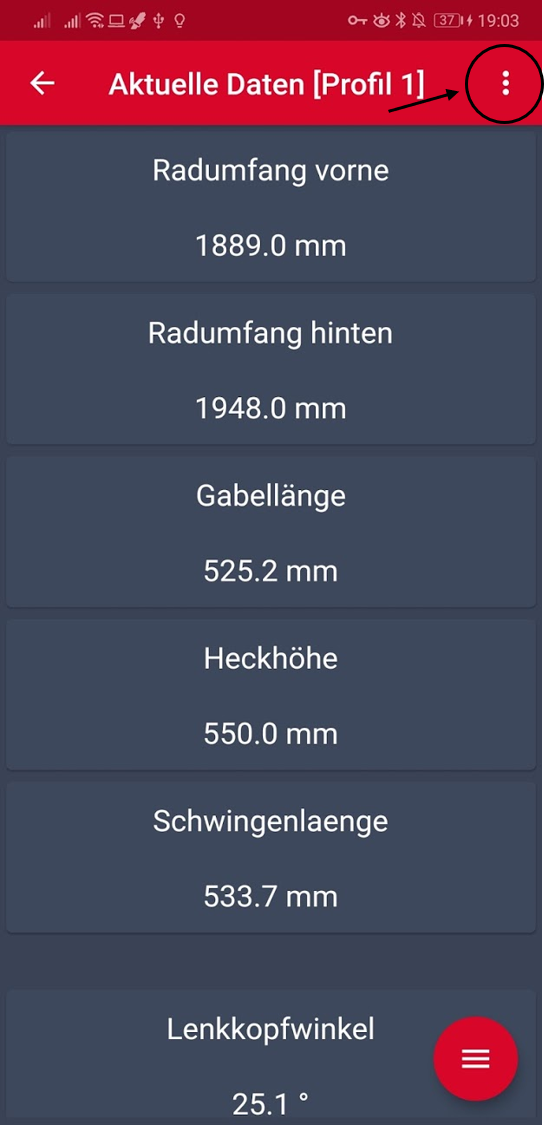
\includegraphics[width=1\textwidth]{../include/images/settings/Open_Settings_02}
	\end{subfigure}
	\hfill
	\begin{subfigure}[b]{0.3\textwidth}
		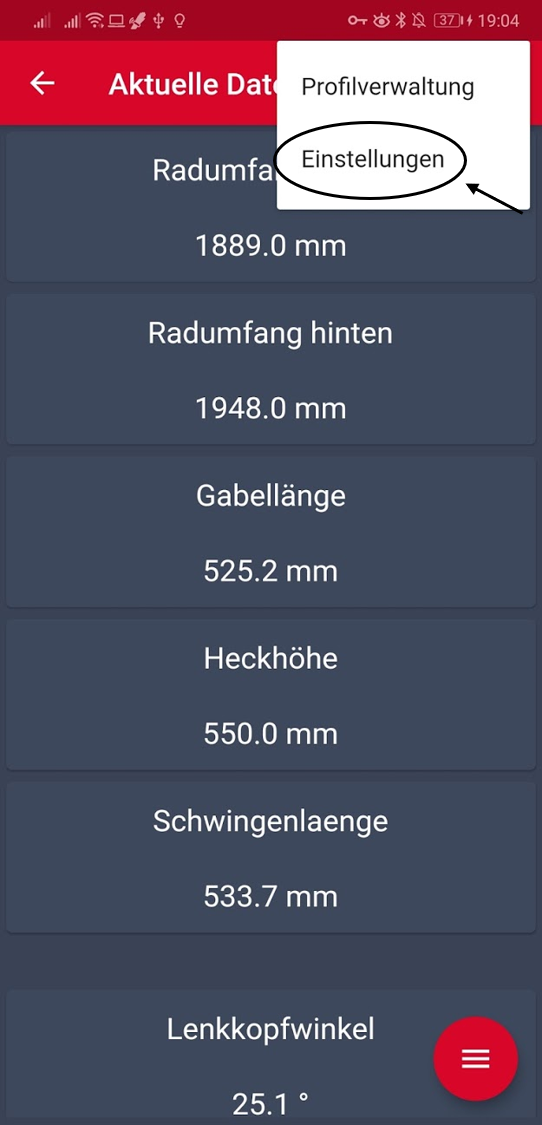
\includegraphics[width=1\textwidth]{../include/images/settings/Open_Settings_03}
	\end{subfigure}
	\caption{Links: Profilverwaltung, Mitte: Button für Dropdown-Menü, Rechts: Dropdown-Menü}
	\label{img:openSettings}
\end{figure}

	\section{Sprache}
	\label{sec:lang}
	
	Die App ist in den Sprachen Deutsch und Englisch verfügbar. Die Einstellung wird standardmäßig auf die im Gerät eingestellte Sprache gesetzt und kann manuell verändert werden (s. \cref{img:settings} rechts)
	
	\section{Eingabemethode}
	\label{sec:input}
	
	Neue Werte, die von der App simuliert werden sollen, werden über die Ansicht "Simulation" eingegeben. Hierfür kann in den Einstellungen angepasst werden, ob die Werte mit Textfeldern oder Slidern eingegeben werden sollen (s. \cref{img:settings} links).
	
	\begin{figure}[H]
		\centering
		\begin{subfigure}[b]{0.45\textwidth}
			\centering
			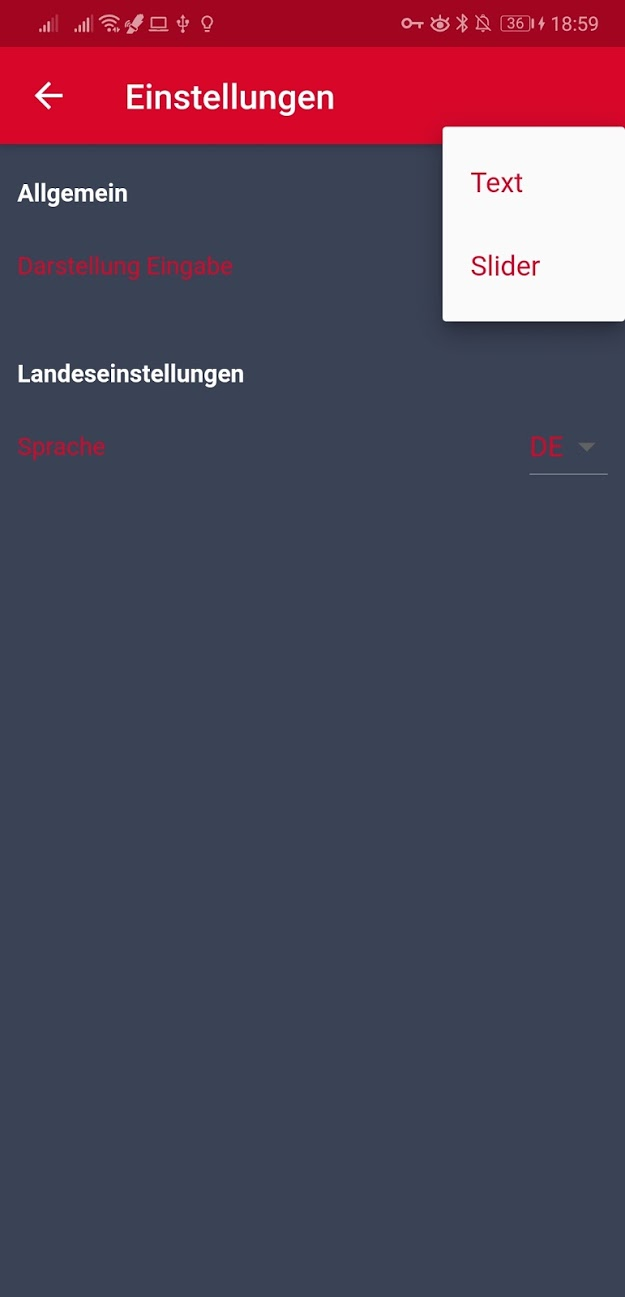
\includegraphics[width=1\textwidth]{../include/images/settings/settings01}
		\end{subfigure}
		\hfill
		\begin{subfigure}[b]{0.45\textwidth}
			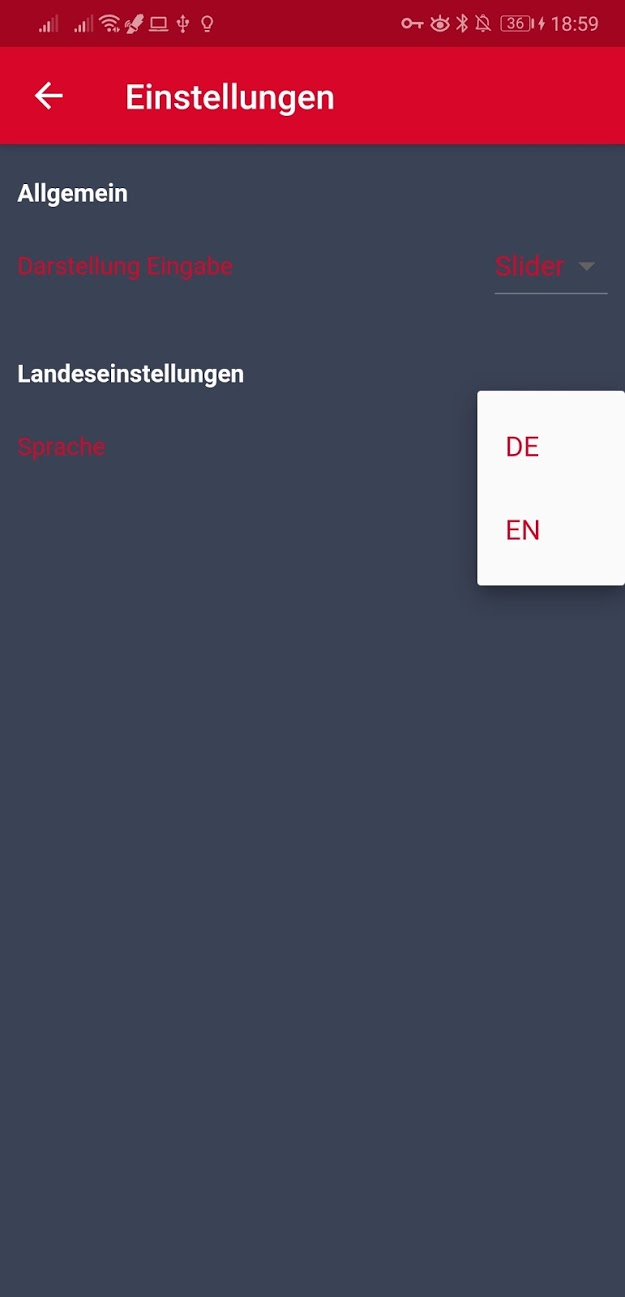
\includegraphics[width=1\textwidth]{../include/images/settings/settings02}
		\end{subfigure}
		\caption{Links: Einstellung der Eingabemethode, Rechts: Einstellung der Sprache}
		\label{img:settings}
	\end{figure}